\documentclass{beamer}

\usetheme{Pittsburgh}
\useinnertheme{default}
\setbeamertemplate{footline}[page number]
\setbeamertemplate{navigation symbols}{}

%\usepackage[utf8]{inputenc}
\usepackage{listings}
\lstset{ %
language=Ruby,                % choose the language of the code
basicstyle=\footnotesize,       % the size of the fonts that are used for the code
numbers=left,                   % where to put the line-numbers
numberstyle=\footnotesize,      % the size of the fonts that are used for the line-numbers
stepnumber=0,                   % the step between two line-numbers. If it's 1 each line 
                                % will be numbered
numbersep=5pt,                  % how far the line-numbers are from the code
backgroundcolor=\color{white},  % choose the background color. You must add \usepackage{color}
showspaces=false,               % show spaces adding particular underscores
showstringspaces=false,         % underline spaces within strings
showtabs=false,                 % show tabs within strings adding particular underscores
frame=none,	                % adds a frame around the code
tabsize=2,	                % sets default tabsize to 2 spaces
captionpos=b,                   % sets the caption-position to bottom
breaklines=true,                % sets automatic line breaking
breakatwhitespace=false,        % sets if automatic breaks should only happen at whitespace
title=\lstname,                 % show the filename of files included with \lstinputlisting;
                                % also try caption instead of title
escapeinside={\%*}{*)},         % if you want to add a comment within your code
emph={add,output,input,icecast,playlist,file,
              fallback,crossfade,http,fade,initial,final,cross},            % if you want to add more keywords to the set
emphstyle=\color[rgb]{0,0.5,0.3},
keywordstyle=\color{red},
stringstyle=\color{blue},
}

\newcommand{\kw}[1]{{\color[rgb]{0,0.5,0.3} #1}}

\usepackage{tikz}
\usepackage[all]{xy}

\renewcommand{\emph}[1]{\alert{#1}}
\renewcommand{\textbf}[1]{{\color{blue} #1}}

%\newtheorem{lemme}{Lemme}
%\newtheorem{theorem}{Theorem}
\newtheorem{proposition}{Proposition}
%\theoremstyle{definition}
%\newtheorem{definition}{Definition}

% \author{David Baelde for Savonet}
\title{\emph{\LARGE Liquidsoap} \\
  A Programming Language for \\ Multimedia Streaming}
\date{David Baelde for Savonet} % 23 Oct 2010, Test Signals, Berlin}

\begin{document}

\begin{frame}
  \maketitle
\end{frame}

\begin{frame}

\vfill

\begin{center}
{\LARGE
Simple things should be simple, \\[1ex]
Complex things should be possible.
}
\begin{flushright}
Alan Kay \hspace{0.5cm} ~
\end{flushright}
\end{center}

\vfill

\end{frame}

%% ===========================================

\begin{frame}[fragile]{Simple things}

\begin{lstlisting}
output.icecast(%vorbis,
               mount="radio.ogg",
               playlist("music.pls"))
\end{lstlisting}

\end{frame}

%% ===========================================

\begin{frame}{Complex things}

\begin{block}{Radio Pi}
\begin{itemize}
\item \emph{Several channels}: jazz, rock, techno, metal, etc.
\item Main channel relaying thematic ones depending on the time
\item \emph{Several outputs per channel}, various bitrates and formats
\item Interface with a web-based \emph{file scheduler}
\item \emph{Live shows} selectively relayed on various thematic channels
\item Volume normalization using \emph{Replay Gain}
\item Smart \emph{cross-fading}
\item \emph{Blank detection} for live and files
\item etc.
\end{itemize}
All this in \emph{one instance} of liquidsoap.
\end{block}

\end{frame}

%% ===========================================

\begin{frame}{Recipe}

\begin{block}{Liquidsoap}
\begin{enumerate}
\item<3-> A script language
\item A notion of source (interactive stream generator)
\item<2-> Interfaces: libraries, external and remote applications
\end{enumerate}
\end{block}

\end{frame}

%% ===========================================

\begin{frame}[fragile]{Designing a stream}

\[
\hspace{-0.4cm}\xymatrix{
  *+[F]{\mathtt{input.http}} \ar[r] &
     *+[F]{\mathtt{fallback}}\ar[r] &
     *+[F]{\mathtt{crossfade}} \ar[r]\ar[dr] &
     *+[F]{\mathtt{output.icecast}} \\
  *+[F]{\mathtt{playlist}}\ar[ur] & & &
     *+[F]{\mathtt{output.file}}\\
}
\]

\vfill
\pause

\begin{lstlisting}
live = input.http("http://server:8000/live.ogg")
music = playlist("/path/to/music")
s = fallback([live,music])
s = crossfade(s)
output.icecast(%vorbis,mount="radio.ogg",s)
output.file(%vorbis,"backup.ogg",s)
\end{lstlisting}

\end{frame}

%% ===========================================

\begin{frame}{Language design}

\begin{block}{Expressiveness vs Safety}

Users should have access to the model:
\begin{itemize}
\item Compose an operator with any sources
\end{itemize}

The language should avoid mistakes:
\begin{itemize}
\item Typos, type errors
\end{itemize}

Key techniques:
\begin{itemize}
\item Static types, inference
\item Functional language: immutability by default
\item Various analyses: fallibility, branching, \ldots
\end{itemize}

\end{block}

\end{frame}

%% ===========================================

\begin{frame}[fragile]{Transitions}

 \begin{center}
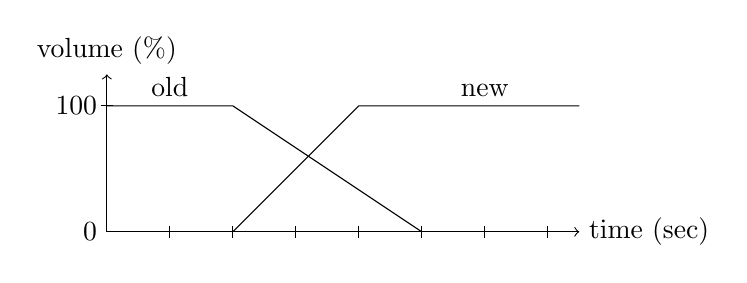
\begin{tikzpicture}[xscale=0.8,yscale=0.8]
\draw[->] (0,0) -- (0,2.5);
\draw (-0.1,2) -- (0.1,2);
\draw (0,2) node[anchor=east]{100};
\draw (0,0) node[anchor=east]{0};
\draw[->] (0,0) -- (7.5,0);
\foreach \x in {1,2,3,4,5,6,7} \draw (\x,-0.1) -- (\x,0.1);
\draw (0,2.5) node[anchor=south]{volume (\%)};
\draw (7.5,0) node[anchor=west]{time (sec)};
\draw (0,2) -- (2,2) -- (5,0);
\draw (2,0) -- (4,2) -- (7.5,2);
\draw (1,2) node[anchor=south]{old};
\draw (6,2) node[anchor=south]{new};
\end{tikzpicture}
\end{center}

\vfill
\pause

\begin{lstlisting}
def mycross(old,new) =
  add([fade.initial(duration=2.,new),
       fade.final(duration=3.,old)])
end
s = cross(mycross,s)
\end{lstlisting}

\end{frame}

%% ===========================================

\begin{frame}{Features}

\begin{block}{Operators}
\begin{itemize}
\item Play a \kw{single} file, a \kw{playlist} or a queue of files
\item Play a file given by an external script
\item Switch, sequence, add
\item Sound processing: compression, change pitch, etc.
\item Event handlers: tracks, metadata, blank
\end{itemize}
\end{block}

\begin{block}{Interfaces}
\begin{itemize}
\item Icecast, Shoutcast and compatible: output, relay and host
\item ALSA, AO, Pulseaudio, Jack, etc.
\end{itemize}
\end{block}

\textbf{Formats:} WAV, Ogg, MP3, AAC+, Flac, external

\textbf{Also}: requests and protocols, server, etc.

\end{frame}

%% ============================================

\begin{frame}{Does it make coffee?}
\vfill
\begin{center}
{\LARGE No} ~ (not even the sound of brewing it)
\end{center}
\vfill

It also does not have
\begin{itemize}
\item any comprehensive graphical interface,
\item web interface,
\item or any kind of database integration.
\end{itemize}
\end{frame}

\begin{frame}{The price to pay}

\begin{block}{Everything has to be decoded}
The model allowing arbitrary compositions \\
makes it difficult to avoid decoding.
\end{block}

\vfill\pause

\begin{block}{But that's all!}
It's even efficient:
\begin{itemize}
\item competes with \texttt{ices} on similar tasks
\item 80 instances on a single Core i7 920
\end{itemize}
\end{block}

\end{frame}

\begin{frame}{Related tools}

To name a few: chuck, puredata, faust, streamit \ldots

\vfill

We have more high-level notions: track, metadata \\
and an \emph{interactive} notion of source \\
and many other nice ``auxiliary'' things (request, server).

\end{frame}

%% ===========================================

\begin{frame}{Stream content}
Stream content and conversions: montrer ça du point de vue audio, les applis usuelles ne permettent en effet pas de controler ce genre de chose (c'est plus un truc de lib genre gstreamer ou jack); peut etre parler de video et midi.
\end{frame}

%% ===========================================

\begin{frame}{Clocks}
General idea, external and internal motivations (cross, drift and lags)
\end{frame}

%% ===========================================

\begin{frame}{Background}

\begin{block}{The Savonet team}
Since 2003 \\
Main devs: David Baelde, Romain Beauxis and Samuel Mimram. \\
A few others: Peter Brookes, Vincent Tabard, etc.
\end{block}

\begin{block}{Programming languages}
Mostly OCaml (pros and a little cons for contributors)
\end{block}

\begin{block}{A noble goal}
Bringing research ideas and tools to the masses!
\end{block}

\end{frame}

%% ===========================================

\begin{frame}{Conclusion}

\begin{block}{Liquidsoap}
\begin{itemize}
\item More features than most tools
\item A unique ability to combine them at will
\end{itemize}
\end{block}

\begin{block}{Future}
\begin{itemize}
\item Already there: video and MIDI streams
\item Coming: more real-time uses, e.g. telephony
\end{itemize}
\end{block}

\begin{block}{Community}
If you like it, contribute, even if you don't know how to code in
OCaml, or don't code at all.
\end{block}

\end{frame}

\end{document}
